%!TEX program = xelatex
%!TEX root = Algebra_1.tex
%%Usar makeindex -s indexstyle.ist arquivo.idx no terminal para gerar o índice remissivo agrupado por inicial
%%Após executar pdflatex arquivo
\chapter{Conceitos Básicos} % (fold)
\label{cha:conceitos_basicos}

\begin{definicao}
    Uma \textbf{proposição} é todo conjunto de palavras ou símbolos ao qual podemos atribuir um \textbf{valor lógico}.
\end{definicao}

\begin{definicao}
    Diz-se que o \textbf{valor lógico} de uma proposição é ``verdade'' (V) se a proposição é verdadeira ou ``falsidade'' (F) se a proposição é falsa.
\end{definicao}

\begin{exemplos}
    Julgue se as seguintes sentenças são ou não proposições:
    \begin{enumerate}[label={\arabic*})]
        \item Todo número primo é ímpar.
        \begin{solucao}
            Essa setença é uma proposição de valor lógico "Falsidade."
        \end{solucao}

        \item $x^2 + y^2 \ge 0$ para todos $x$, $y \in \real$.
        \begin{solucao}
            Esse setença é uma proposição de valor lógico "Verdade".
        \end{solucao}

        \item Amanhã irá chover.
        \begin{solucao}
            Essa sentença não é uma proposição. Não é possível atribuir um valor lógico a ela.
        \end{solucao}
    \end{enumerate}

\end{exemplos}

\section{Princípio da não contradição e do terceiro excluído} % (fold)
\label{sec:principio_da_nao_contradicao_e_do_3}
\begin{enumerate}[label={\roman*})]
    \item Uma proposição não pode ser verdadeira e falsa ao mesmo tempo.
    \item Toda proposição ou é verdadeira ou é falsa, isto é, verifica-se sempre um destes casos e nunca um terceiro.
\end{enumerate}

Assim esses princípios afirmam que:
\begin{center}
    ``Toda proposição tem um, e um só, dos valores lógicos \textbf{verdade} ou \textbf{falsidade}.''
\end{center}

De modo geral vamos trabalhar com proposições da forma:
\begin{enumerate}[label={\roman*})]
    \item Se $\mathbb{H}$, então $\mathbb{T}$.

    Aqui $\mathbb{H}$ é chamado de hipótese e $\mathbb{T}$ de tese. Neste tipo de proposição iremos admitir que $\mathbb{H}$ é uma verdade e precisaremos provar que $\mathbb{T}$ é verdade. Ou seja precisamos construir um argumento que justifique $\mathbb{T}$ ser verdadeira à partir do fato de $\mathbb{H}$ ser verdadeira.

    \item $\mathbb{H}$ se, e somente se, $\mathbb{T}$ ou $\mathbb{H}$ se, e só se, $\mathbb{T}$.

    Esse tipo de proposição será decomposta em duas proposições no formato anterior. Isto é:
    \begin{enumerate}[label={\alph*})]
        \item Se $\mathbb{H}$, então $\mathbb{T}$.
        \item Se $\mathbb{T}$, então $\mathbb{H}$.
    \end{enumerate}

    No primeiro caso admitimos $\mathbb{H}$ verdadeira e provamos que $\mathbb{T}$ também é verdadeira e no segundo caso admitimos que $\mathbb{T}$ é verdadeira e provamos que $\mathbb{H}$ é verdadeira.
\end{enumerate}

Para demonstrarmos uma proposição precisamos deduzí-la de proposições previamente comprovadas como verdadeiras. Assim uma demonstração é a determinação de uma verdade e é construída através de uma sequência de raciocínios lógicos, com início e fim determinados. Cada passo dessa sequência de raciocínio deve ter sua veracidade justificada, seja através de outras proposições já provadas verdadeiras ou pelo uso de axiomas, que são afirmações admitidas como verdadeiras. Vamos utilizar, principalmente, três formas de demonstrar uma proposição, a saber:
\begin{enumerate}[label={\roman*})]
    \item Demonstração direta;
    \item Demonstração por contraposição;
    \item Demonstração por contradição ou redução ao absurdo.
\end{enumerate}

Assim numa proposição do tipo:
\begin{center}
    Se $\mathbb{H}$, então $\mathbb{T}$.
\end{center}

Para demonstrá-la de forma \textbf{direta} devemos admitir que a hipótese $\mathbb{H}$ é \textbf{verdadeira} e, utilizando de uma sequência de passos
cuja veracidade podemos comprovar, chegar à conclusão que a tese $\mathbb{T}$ também é \textbf{verdadeira}.

Na \textbf{demonstração por contraposição}, iremos supor que a tese $\mathbb{T}$ é \textbf{falsa} e novamente através de uma
sequência de passos que podemos justificar como verdadeiros, devemos chegar à conclusão que a hipótese $\mathbb{H}$ também é
\textbf{falsa}. Se conseguirmos chegar a essa conclusão então a proposição original será \textbf{verdadeira}.

Por último, na \textbf{demonstração pro contradição} ou \textbf{redução ao absurdo}, iremos admitir que a hipótese
$\mathbb{H}$ é \textbf{verdadeira} e que a tese $\mathbb{T}$ é \textbf{falsa}. Usando essas suposições devemos chegar à alguma
conclusão contraditória, isto é, precisamos obter alguma informação que seja verdadeira e falsa ao mesmo tempo. Nesse caso,
significa que nossa tese $\mathbb{T}$ deve ser obrigatoriamente \textbf{verdadeira}, e com isso a proposição também será
\textbf{verdadeira}.

% section príncipio_da_não_contradição_e_do_3 (end)

% chapter conceitos_básicos (end)

\chapter{Noções de Teoria de Conjuntos}
\section{Conceitos básicos}

Um conjunto é uma ``coleção'' ou ``família'' de elementos.

Usaremos letras maiúsculas do alfabeto para denotar os conjuntos e denotaremos elementos de um dado conjunto por letras minúsculas do alfabeto.

Dado um conjunto $A$, para indicar o fato de que $x$ é um elemento de $A$, escrevemos:
\[
    x \in A.
\]

Para dizer que um elemento $x$ não pertence ao conjunto $A$, escrevemos:
\[
    x \notin A.
\]

Um conjunto sem elementos é chamado de \textbf{conjunto vazio}. Tal conjunto é denotado por $\emptyset$ ou por $\{\ \}$.

Dado um conjunto $A$ e $x$ um elemento, ocorre sempre uma das seguintes situações:
\[
    x \in A \mbox{ ou } x \notin A.
\]

Além disso, para dois elementos $x$, $y \in A$, ocorre exatamente uma das seguinte situações:
\[
    x = y \mbox{ ou } x \neq y.
\]

\section{Descrição de um conjunto}

Um conjunto $A$ pode ser dado pela simples listagem dos seus elementos, como por exemplo:
\begin{align*}
    A &= \{1,2,3,4,5\}\\
    B &= \{verdade, falso\}.
\end{align*}

Um conjunto também pode ser dado pela descrição das propriedades dos seus elementos, como por exemplo:
\[
    A = \{\mbox{números naturais\ } n \mid n \mbox{ é múltiplo de } 2\} = \{2,4,6,...\}.
\]

\section{Alguns conjuntos importantes}
\begin{enumerate}[label={\arabic*})]
    \item $\n = \{0,1,2,3,...\}$ o conjunto dos números naturais.
    \item $\n_0 = \{0,1,2,3,...\}$ o conjunto dos números inteiros não negativos.
    \item $\z = \{...,-2,-1,0,1,2,...\}$ o conjunto dos números inteiros.
    \item $\rac = \left\{\dfrac{p}{q} \mid p,q \in \z, q \neq 0 \right\}$ o conjunto dos números racionais.
    \item $\real $ o conjunto dos números reais.
    \item $\real^*$ o conjunto dos números reais não nulos.
    \item $\complex = \{a + bi \mid a,b \in \real,\ i^2 = -1\}$ o conjunto dos números complexos.
\end{enumerate}

\begin{observacao}
    Para esses conjuntos vamos admitir como verdadeiras as propriedades básicas da soma e multiplicação.
\end{observacao}
\section{Propriedades dos conjuntos}

\begin{definicao}\label{igualdade_conjuntos}
    Dados dois conjuntos $A$ e $B$, dizemos que $A$ e $B$ são \textbf{iguais} se, e somente se, eles têm os mesmos elementos. Ou seja, para todo $x \in A$ também vale que $x \in B$ e para todo $y \in B$ também vale que $y \in A$. Se $A$ e $B$ são iguais, escrevemos $A = B$.
\end{definicao}

\begin{exemplo}
    Sejam $A = \{1,1,2,3,4,4\}$, $B = \{3,2,1,4\}$, $C = \{1,2,3\}$ e $D = \{2,3\}$. Então de acordo com a Definição
    \ref{igualdade_conjuntos} temos $A = B$ pois todo elemento de $A$ está em $B$ e todo elemento de $B$ também está em $A$. Agora
    como $1 \in C$ e $1 \notin D$, então $C \ne D$.
\end{exemplo}

\begin{observacao}
    Dados conjuntos $A$ e $B$, de acordo com a Definição \ref{igualdade_conjuntos} para que $A \ne B$ basta que exista um elemento $x \in A$ de maneira que $x \notin B$ ou que exista $y \in B$ com a condição de que $y \notin A$.
\end{observacao}

\begin{definicao}\label{definicao_continencia_conjuntos}
    Se $A$ e $B$ são dois conjuntos, dizemos que $A$ é um \textbf{subconjunto} de $B$ ou que $A$ \textbf{está contido} em $B$ ou que $B$ \textbf{contém} $A$ se todo elemento de $A$ for elemento de $B$. Ou seja, se para todo elemento $x \in A$, temos $x \in B$. Nesse caso, escrevemos $A \subseteq B$ (ou $A \subset B$) ou $B \supseteq A$ (ou $B \supset A$).
\end{definicao}


Caso $A$ seja um subconjunto de $B$ mas não é igual a $B$, escrevemos:
\[
    A \subsetneq B.
\]

Nesse caso, dizemos que $A$ é um \textbf{subconjunto pr{ó}prio} de $B$.

\begin{exemplos}
    Sejam $A = \{1,2,3,x,y,z\}$, $B = \{x, y\}$ e $C = \{x, y , z\}$. Temos:
    \begin{enumerate}[label={\arabic*})]
        \item $A \nsubseteq B$ pois $1 \in A$ e $1 \notin B$.
        \item $B \subsetneq A$ pois todo elemento de $B$ também está em $A$. Observe que existem elementos de $A$ que não estão em $B$, por exemplo $2 \in A$ e $2 \notin B$.
        \item $B \subseteq C$ pois todo elemento de $B$ também está em $C$.
        \item $C \subseteq A$ pois todo elemento de $C$ também está em $A$.
    \end{enumerate}
\end{exemplos}

\begin{observacao}
    Dados dois conjuntos $A$ e $B$ pela Definição \ref{definicao_continencia_conjuntos} para que $A$ \textbf{não esteja contido em} $B$ basta que exista $x \in A$ tal que $x \notin B$. Nesse caso escrevemos $A \nsubseteq B$.
\end{observacao}

Usando a definição de continência de conjuntos, Definição \ref{definicao_continencia_conjuntos}, podemos redefinir a igualdade de conjuntos, Definição \ref{igualdade_conjuntos}, da seguinte forma: dados dois conjuntos $A$ e $B$
\begin{center}
    $A = B$\quad \textbf{se, e somente se,}\quad $A \subseteq B$\quad \textbf{e}\quad $B \subseteq A$.
\end{center}

Ou seja,
\begin{center}
    \textbf{se} $A = B$ \textbf{então} $A \subseteq B$ \textbf{e} $B \subseteq A$.
\end{center}

Além disso,
\begin{center}
    \textbf{se} $A \subseteq B$ \textbf{e} $B \subseteq A$, \textbf{então} $A = B$.
\end{center}

Quando $A$ e $B$ não são iguais, escrevemos $A \neq B$. Para que $A \neq B$ devemos ter $A \nsubseteq B$ ou $B \nsubseteq A$. Isto é, precisamos encontrar algum elemento $x \in A$ de modo que $x \notin B$ ou então encontrar $y \in B$ com a condição de que $y \notin A$.

\begin{proposicao}
    Dados três conjuntos $A$, $B$ e $C$ temos:
    \begin{enumerate}[label={\roman*})]
        \item $A\subseteq A$ (Reflexividade)
        \item Se $A\subseteq B \mbox{ e } B\subseteq A$, então $A=B$. (Antissimetria)
        \item Se $A\subseteq B$ e $B\subseteq C$, então $A\subseteq C$. (Transitividade)
    \end{enumerate}
\end{proposicao}


Considere os seguintes conjuntos:
\begin{align*}
    A &= \{ n \in \n \mid n \mbox{ é múltiplo de } 2\} = \{2,4,6,...\}\\
    B &= \{n \in \n \mid n \mbox{ é múltiplo de } 3\} = \{3,6,9,...\}.
\end{align*}


Neste caso, $2 \in A$ e $2 \notin B$, logo $A \nsubseteq B$. Por outro lado, $3 \in B$ e $3 \notin A$ e com isso $B \nsubseteq A$. Portanto, dados dois conjuntos $A$ e $B$, nem sempre temos $A \subseteq B$ ou $B \subseteq A$.

\begin{proposicao}
    Seja $A$ um conjunto. Então $ \emptyset \subseteq A$.
\end{proposicao}
\begin{prova}
    Suponha que $\emptyset \nsubseteq A$. Logo existe $x \in \emptyset$ tal que $x \notin A$. Mas por definição, o conjunto vazio não contém elementos. Logo a existência de $x \in \emptyset$ é uma contradição. Tal contradição surgiu por termos suposto que $\emptyset \nsubseteq A$. Portanto, $\emptyset \subseteq A$, como queríamos demonstrar.
\end{prova}

\section{Relações entre conjuntos}

\begin{definicao}\label{intersecao_conjunto}
    Sejam $A$ e $B$ dois conjuntos. Definimos a \textbf{intersecção} de $A$ e $B$ como sendo o conjunto $A \cap B$ cujos elementos pertencem aos conjuntos $A$ e $B$ simultaneamente. Assim,
    \[
        A \cap B = \{x \mid x \in A\mbox{ e }  x \in B\}.
    \]

    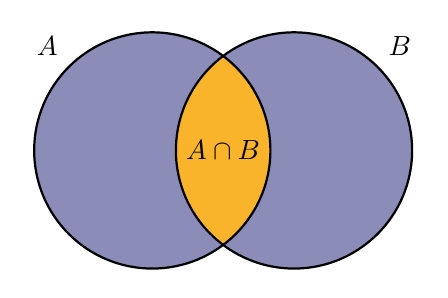
\begin{tikzpicture}[thick,
    set/.style = {circle,
        minimum size = 3cm,
        fill=MidnightBlue!50}]

% Set A
\node[set,label={135:$A$}] (A) at (0,0) {};

% Set B
\node[set,label={45:$B$}] (B) at (1.8,0) {};

% Intersection
\begin{scope}
    \clip (0,0) circle(1.5cm);
    \clip (1.8,0) circle(1.5cm);
    \fill[Dandelion](0,0) circle(1.5cm);
\end{scope}

% Circles outline
\draw (0,0) circle(1.5cm);
\draw (1.8,0) circle(1.5cm);

% Set intersection label
\node at (0.9,0) {$A\cap B$};

\end{tikzpicture}
\end{definicao}

\begin{exemplo}
    Sejam $A = \{1, 2, 3\}$, $B = \{2, 3, 4\}$ e $C = \{r, s, t\}$. Então
    \begin{align*}
        A \cap B &= \{2, 3\}\\
        A \cap C &= \emptyset.
    \end{align*}
\end{exemplo}

\begin{definicao}\label{unicao_conjuntos}
    Sejam $A$ e $B$ dois conjuntos. Definimos a \textbf{união} de $A$ com $B$ como sendo o conjunto $A \cup B$, cujos elementos pertencem ao conjunto $A$ ou ao conjunto $B$. Assim,
    \[
        A \cup B = \{x \mid x \in A \mbox{ ou } x \in B\}.
    \]

    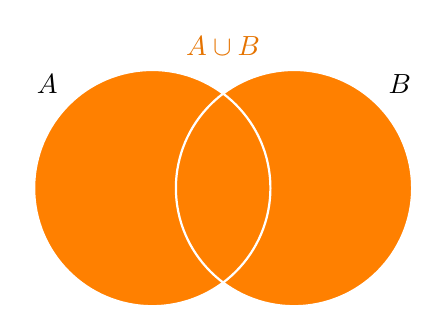
\begin{tikzpicture}[thick,set/.style = {circle,fill=orange,minimum size =3cm}]

        % Set A
        \node [set,label={135:$A$}] (A) at (0,0){};

        % Set B
        \node [set,label={45:$B$}] (B) at (1.8,0){};

        % Circles outline
        \draw[white] (0,0) circle(1.5cm);
        \draw[white] (1.8,0) circle(1.5cm);

        % Union text label
        \node[orange!90!black] at (0.9,1.8) {$A\cup B$};

    \end{tikzpicture}
\end{definicao}

\begin{exemplo}
    Sejam $A = \{1, 2, 3\}$, $B = \{2, 3, 4\}$ e $C = \{r, s, t\}$. Então
    \begin{align*}
        A \cup B &= \{1,2,3,4\}\\
        A \cup C &= \{1,2,3,r,s,t\}.
    \end{align*}
\end{exemplo}

\begin{proposicao} Sejam $A$ e $B$ dois conjuntos. Então:
    \begin{enumerate}[label={\roman*})]
        \item $(A \cap B) \subseteq A$;
        \item $(A \cap B) \subseteq B$;
        \item $A \subseteq A \cup B$;
        \item $B \subseteq A \cup B$.
    \end{enumerate}
\end{proposicao}
\begin{prova}
    Para provar a primeira afirmação seja $x \in A \cap B$ um elemento qualquer. Da definição de interseção de conjuntos, Definição \ref{intersecao_conjunto}, temos $x \in A$ e $x \in B$. Assim podemos afirmar com certeza que $x \in A$. Logo todo elemente de $A \cap B$ também está em $A$, ou seja, $A \cap B \subseteq A$. De modo análogo prova-se a segunda afirmação sobre a interseção.

    Para a terceira afirmação, seja $x \in A$. Da definição de união de conjuntos, Definição \ref{unicao_conjuntos}, segue que $x \in A \cup B$. Logo todo elemento de $A$ também está em $A \cup B$, ou seja, $A \subseteq (A \cup B)$. De modo análogo prova-se a quarta afirmação.
\end{prova}

O conceito de união ($ \cup $) e intersecção ($ \cap $) pode ser estendido para mais de dois conjuntos.

\begin{definicao}
    Sejam $A_{1}$, \dots, $A_{n}$ conjuntos. Então
    \[
        A_{1} \cup A_{2} \cup \cdots \cup A_{n}= \displaystyle\bigcup_{k=1}^n A_{k}
    \]
    é o conjunto dos elementos $x$ tais que $x$ pertence a pelo menos um dos conjuntos $A_{1}$, \dots, $A_{n}$. Agora,
    \[
        A_{1} \cap \cdots \cap A_{n} = \displaystyle\bigcap_{k=1}^{n}A_{k}
    \]
    é o conjunto dos elementos $x$ que pertencem a todos os conjuntos $A_{1}$, \dots, $A_{n}$ simultaneamente.
\end{definicao}

\begin{definicao}
    Sejam $A$ e $B$ conjuntos. Se $A \cap B = \emptyset$, dizemos que $A$ e $B$ são \textbf{conjuntos disjuntos}.
\end{definicao}


Sejam $A$ e $B$ conjuntos tais que $C = A \cup B$ e $A \cap B = \emptyset$. Neste caso dizemos que $C$ é uma \textbf{união disjunta} de $A$ e $B$. Denotamos tal fato por
\[
    C = A \sqcup B.
\]

\begin{proposicao} Sejam $A,\ B$ e $C$ três conjuntos, então:
    \begin{enumerate}[label={\roman*})]
        \item $A \cap (B \cup C) = (A \cap B) \cup (A \cap C)$
        \item $A \cup (B \cap C) = (A \cup B) \cap (A \cup C)$.
    \end{enumerate}
\end{proposicao}
\begin{prova}
    \begin{enumerate}[label={\roman*})]
        \item Precisamos mostrar que
        \begin{enumerate}[label=({\arabic*})]
            \item $A\cap(B\cup C)\subseteq(A\cap B)\cup(A\cap C)$;\label{intersecao_unicao_1}
            \item $(A\cap B)\cup(A\cap C)\subseteq A\cap(B\cup C).$\label{intersecao_unicao_2}
        \end{enumerate}

        Para provar \ref{intersecao_unicao_1} seja $x\in A \cap (B \cup C)$. Logo $x\in A$ e $x\in B\cup C$. Agora, de $x\in B\cup C$, segue que $x\in B$ ou $x\in C$. Suponha que $x\in B$. Como $x\in A$ e $x \in B$, então $x\in A\cap B$. Assim, $x\in(A\cap B)\cup(A\cap C)$, ou seja, $A\cap(B\cup C)\subseteq(A\cap B)\cup(A\cap C)$. Por outro lado, se $x\in C$, como $x\in A$, então $x\in A\cap C$ e daí $x\in(A\cap B)\cup(A\cap C)$, logo $A\cap(B\cup C)\subseteq(A\cap B)\cup(A\cap C)$.

        Portanto,
        \[
            A\cap(B\cup C)\subseteq(A\cap B)\cup(A\cap C).
        \]

        Agora para provar \ref{intersecao_unicao_2}, seja $x\in(A\cap B)\cup(A\cap C)$. Daí, $x\in A\cap B$ ou $x\in A\cap C$. Suponha que $x\in A\cap B$. Assim, $x\in A$ e $x\in B$. Como $x\in B$, segue que $x\in B\cup C$ e então $x\in A\cap(B\cup C)$, ou seja, $(A\cap B)\cup(A\cap C)\subseteq A\cap(B\cup C)$. Agora, suponha que $x\in A\cap C$. Com isso $x\in A$ e $x\in C$. Desse modo, $x\in B\cup C$ e então $x\in A\cap(B\cup C)$ e daí
        \[
            (A\cap B)\cup(A\cap C)\subseteq A\cap(B\cup C).
        \]

        Portanto
        \[
            A\cap(B\cup C)=(A\cap B)\cup(A\cap C),
        \]
        como queríamos.
        \item Análoga ao caso anterior.
    \end{enumerate}
\end{prova}

\begin{definicao}
    Dados dois conjuntos $A$ e $B$, definimos a \textbf{diferença} dos conjuntos $A$ e $B$, denotada por $A-B$ ou $A\backslash B$ como sendo o conjunto
    \[
        A - B = \{x \mid x \in A \mbox{ e } x \notin B\}.
    \]

    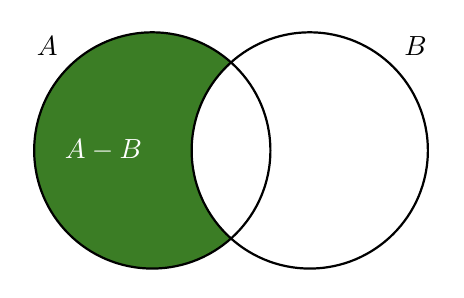
\begin{tikzpicture}[thick,set/.style = { circle, minimum size = 3cm}]

        % Set A
        \node[set,fill=OliveGreen,label={135:$A$}] (A) at (0,0) {};

        % Set B
        \node[set,fill=white,label={45:$B$}] (B) at (0:2) {};

        % Circles outline
        \draw (0,0) circle(1.5cm);
        \draw (2,0) circle(1.5cm);

        % Difference text label
        \node[left,white] at (A.center){$A-B$};

    \end{tikzpicture}
\end{definicao}

\begin{exemplos}
    \begin{enumerate}[label={\arabic*})]
        \item Se $A=\{1,2,3,5,4\}$, $B=\{2,3,6,8\}$, então
        \begin{align*}
            A - B &= \{1,4,5\}\\
            B - A &=\{6,8\}.
        \end{align*}
        \item Se $A=\{2,4,6,8,10,...\}$, $B=\{3,6,9,12,15,...\}$, então
        \begin{align*}
             A - B &= \{2,4,8,10,14,16,...\}\\
             B - A &= \{3,9,15,21,...\}
         \end{align*}
    \end{enumerate}

\end{exemplos}

\begin{proposicao}
    Sejam $A$, $B$ e $C$ conjuntos não vazios. Então
    \[
        (A \cup B) - C = (A - C) \cup (B - C).
    \]
\end{proposicao}
\begin{prova}
    Precisamos mostrar que
    \begin{enumerate}[label={\arabic*})]
        \item $(A \cup B) - C \sub (A - C) \cup (B - C)$
        \item $(B - C) \sub (A \cup B) - C = (A - C)$
    \end{enumerate}
    Para a primeira inclusão seja $x \in (A \cup B) - C$. Assim por definição, $x \in A \cup B$ e $x \notin C$. De $x \in A \cup B$, então $x \in A$ ou $x \in B$.

    Se $x \in A$, como $x \notin C$ segue então que $x \in A - C$. Logo $x \in (A - C) \cup (B - C)$.

    Se $x \in B$, como $x \notin C$ segue então que $x \in B - C$. Logo $x \in (A - C) \cup (B - C)$.

    Assim $(A \cup B) - C = (A - C) \sub (B - C)$.

    Agora, para a segunda inclusão, seja $y \in (A - C) \cup (B - C)$. Por definição, $x \in A - C$ ou $x \in B - C$.

    Se $x \in A - C$, então $x \in A$ e $x \notin C$. Como $x \in A$, segue que $x \in A \cup B$. Mas $x \notin C$, com isso, $x \in (A \cup B) - C$.

    Se $x \in B - C$, então $x \in B$ e $x \notin C$. Como $x \in B$, segue que $x \in A \cup B$. Mas $x \notin C$, com isso, $x \in (A \cup B) - C$.
    Assim $(A - B) \cup (B - C) \sub (A \cup B) - C$.

    Portanto, $(A \cup B) - C = (A - C) \cup (B - C)$, como queríamos.
\end{prova}

\begin{definicao}
    Dados dois conjuntos $A$ e $E$ tais que $A\subseteq E$, definimos o \textbf{complementar} de $A$ em $E$, denotado $A^C$ ou $C_E(A)$, como
    \[
        C_E(A) = \{ x \in E \mid x \notin A \}.
    \]

    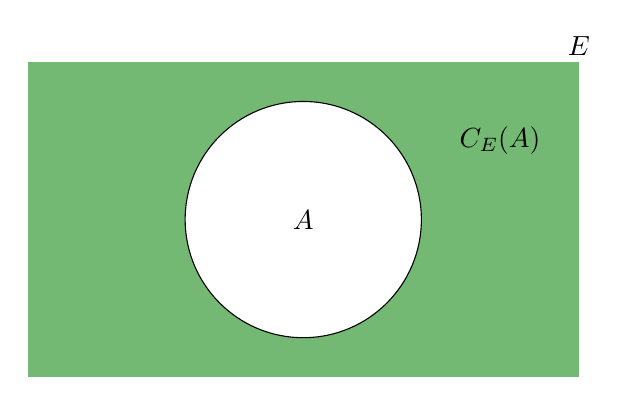
\begin{tikzpicture}
        \fill[Green!55!white, even odd rule](5,-2) rectangle (-2,2) (0:2cm);
        \fill[white] (1.5, 0) circle[radius=1.5];
        \draw[black] (1.5, 0) circle [radius=1.5];

        \node at (1.5, 0) (A) {$A$};
        \node at (4, 1) (C) {$C_E(A)$};
        \node at (5, 2.2) (E) {$E$};
    \end{tikzpicture}
\end{definicao}

\begin{observacoes}
    \begin{enumerate}[label={\arabic*})]
        \item Se $A = E$, então $C_A(A) = \{ x \in A \mid x \notin A \} = \emptyset$.
        \item $(A^C)^C = \{x \in E \mid x \notin A^C\} = \{ x \in E \mid x \in A \} = A$
    \end{enumerate}

\end{observacoes}

\begin{exemplo}
    Sejam $A = \{1,2,3,4\}$ e $E = \{1,2,3,5,4,0,8,9\}$. Primeiro note que $A \subseteq E$, daí
    \[
            A^C = C_E(A) = \{0,5,8,9\}.
    \]
\end{exemplo}

\begin{proposicao}
    Sejam $A$, $B$ e $E$ conjuntos. Se $A\subseteq B\subseteq E$, então $C_E(B)\subseteq C_E(A)$.
\end{proposicao}
\begin{prova}
    Seja $x \in C_E(B)$. Assim $x\notin B$ e como $A \subseteq B$, então $x \notin A$. Daí por definição $x\in C_E(A)$, ou seja, $C_E(B) \subseteq C_E(A)$.
\end{prova}

\begin{proposicao} Sejam $A$, $B$ e $E$ três conjuntos tais que $A\subseteq E$ e $B\subseteq E$. Então:
\begin{enumerate}[label={\roman*})]
    \item $(A\cup B)^C = A^C\cap B^C$
    \item $(A\cap B)^C = A^C\cup B^C$
\end{enumerate}
\end{proposicao}
\begin{prova}
    \begin{enumerate}[label={\roman*})]
        \item Seja $x \in (A\cup B)^C$. Logo $x\notin A\cup B$, assim $x\notin A$ e $x\notin B$. Daí, $x\in A^C$ e $x\in B^C$, isto é, $x\in A^C\cap B^C$. Desse modo,
        \begin{equation}\label{complementar_uniao-1}
            (A\cup B)^C \subseteq A^C\cap B^C.
        \end{equation}

        Por outro lado, se $x\in A^C\cap B^C$, então $x\in A^C$ e $x\in B^C$. Com isso, $x\notin A$ e $x\notin B$, ou seja, $x\notin A\cup B$, logo $x\in (A\cup B)^C$. Desse modo
        \begin{equation}\label{complementar_uniao-2}
            A^C\cap B^C\subseteq(A\cup B)^C.
        \end{equation}

        Portanto, de \eqref{complementar_uniao-1} e \eqref{complementar_uniao-2} temos
        \[
            (A\cup B)^C = A^C\cap B^C.
        \]

        \item Seja $x \in (A\cap B)^C$. Logo $x\notin A\cap B$, assim $x\notin A$ ou $x\notin B$. Então $x\in A^C$ ou $x\in B^C$, isto é, $x\in A^C\cup B^C$. Desse modo,
        \begin{equation}\label{complementar_intersecao-1}
            (A\cap B)^C \subseteq A^C\cup B^C.
        \end{equation}

        Por outro lado, se $x\in A^C\cup B^C$, então $x\in A^C$ ou $x\in B^C$. Daí, $x\notin A$ ou $x\notin B$, ou seja, $x\notin A\cap B$, logo $x\in (A\cap B)^C$. Desse modo
        \begin{equation}\label{complementar_intersecao-2}
            A^C\cup B^C\subseteq(A\cap B)^C.
        \end{equation}

        Portanto, de \eqref{complementar_intersecao-1} e \eqref{complementar_intersecao-2} temos
        \[
            (A\cap B)^C = A^C\cup B^C.
        \]
    \end{enumerate}
\end{prova}

\begin{definicao}
    Dados dois conjuntos $A$ e $B$, definimos o \textbf{produto cartesiano} de $A$ por $B$ como sendo o conjunto
    \[
        A \times B = \{(x,y) \mid x\in A, y\in B\}.
    \]
\end{definicao}

Dados $(x,y)$, $(z,t) \in A\times B$, temos
\begin{center}
    $(x,y) = (z,t)$ \textbf{se, e somente se,} $x = z$ \textbf{e} $y = t$.
\end{center}

\begin{exemplo}\label{exemplo_produto_cartesiano}
    Sejam $A = \{1,2\}$ e $B = \{3,4\}$. Então
    \begin{align*}
        A \times B &= \{(1,3), (1,4), (2,3), (2,4)\}\\
        B \times A &= \{(3,1), (3,2), (4,1), (4,2)\}
\end{align*}
\end{exemplo}

\begin{observacoes}
    \begin{enumerate}[label={\arabic*})]
        \item Do Exemplo \eqref{exemplo_produto_cartesiano} vemos que em geral $A \times B \neq B\times A$.
        \item No caso em que $A = B$ vamos escrever
        \[
            A \times A = A^2 = \{ (x, y) \mid x, y \in A\}.
        \]
        De modo geral:
        \[
            \underbrace{A \times A \times \cdots \times A}_{n\ vezes} = A^n = \{ (x_1, x_2, \dots, x_n) \mid x_1, x_2, \dots, x_n \in A\}
        \]
        para $n \ge 2$.
    \end{enumerate}
\end{observacoes}

\begin{definicao}
    Para qualquer conjunto $A$, indicamos por $\mathcal{P}(A)$ o conjunto
    \[
        \mathcal{P}(A) = \{ X \mid X\subseteq A\}
    \]
    que é chamado de \textbf{conjunto das partes} de $A$.
\end{definicao}

Os elementos desse conjunto são todos os subconjuntos de $A$. Dizer que $Y\in \mathcal{P}(A)$ significa que $Y \subseteq A$. Particularmente, temos $\emptyset\in \mathcal{P}(A)$ e $A\in \mathcal{P}(A)$.

\begin{exemplos}
    \begin{enumerate}[label={\arabic*})]
        \item $A = \emptyset$, $\mathcal{P}(A) = \{\emptyset\}$;
        \item $B = \{x\}$, $\mathcal{P}(B) = \{\emptyset, \{x\}\}$;
        \item $C = \{a,b,c\}$, $\mathcal{P}(C)=\{\emptyset, \{a\}, \{b\},\{c\},\{a,b\},\{a,c\},\{b,c\},C\}$;
        \item $D=\real$, $\mathcal{P}(D)=\{X\mid X \subseteq \real\}$, por exemplo $\rac\in \mathcal{P}(D)$.
    \end{enumerate}
\end{exemplos}
